\documentclass[../main.tex]{subfiles}

\begin{document}

\chapter{Calibrazione modello solare standard}

La luminosit\'a dipende fortemente dal valore di $Y_{in}$,  mentre il raggio da $\alpha$, parametro che regola l'efficienza del trasporto convettivo nella regione esterna.

%dln(L)/d\alpha=0.02
%dlnr/dY=2.1
%dlnr/d\alpha=-0.19

\begin{wraptable}{r}{5.5cm}
\caption{Dipendenza dei parametri del modello $Y_{in}$ e $\alpha$ dalle osservabili.}\label{parametersdeps}
\begin{threeparttable}
\begin{tabular}{c|c}
$\PDly{\midfrac{Z}{X}}{Y}=-0.3$\tnote{1}&$\PDy{\ln{L}}{\alpha}=50$\tnote{2}\\
$\PDly{\agesun{}}{Y}=-0.21$\tnote{1}&$\PDy{\ln{r}}{\alpha}=-5.3$\tnote{2}\\
$\PDy{\ln{r}}{Y}=0.48$\tnote{2}&$$\\
$\PDly{\lsun{}}{Y}=0.4$\tnote{1}&$$\\
$\PDly{S_{11}}{Y}=0.1$\tnote{1}&$$\\
$\PDly{S_{33}}{Y}\leq0.01$\tnote{1}&$$\\
$\PDly{S_{34}}{Y}\leq0.01$\tnote{1}&$$\\
\end{tabular}
\begin{tablenotes}
\item[1] \cite{bahcall1982standard}; \item[2] \cite{stix91sun}
\end{tablenotes}
\end{threeparttable}
\end{wraptable} 

\chapter{Misura campo di velocit\'a solare}

\section{Doppler shift}

\subsection{Resonant scattering spectrometers}

Tacometro di Fourier, 

Hyperfine splitting: scattering polarization component.

\chapter{Descizione Euleriana e Lagrangiana}

\chapter{Convezione}

\chapter{Equazione di stato}

Il teorema del viriale applicato ad un gas autogravitante descritto dall'equazione di stato dei gas perfetti monoatomici, $P=(\gamma-1)\rho u$ con $\gamma=\frac{c_P}{c_V}=\frac{5}{3}$, 
Per un'equazione di stato generale definisco il parametro $\zeta$ che mette in relazione l'energia interna u con la frazione di energia interna dovuta ai moti traslazionali
\begin{align}
&\zeta u=3\frac{P}{\rho}&\intertext{per un gas ideale monoatomico non relativistico}\nonumber\\
&\zeta=3(\gamma-1)\xrightarrow{\gamma=\frac{5}{3}}2
\end{align}


\chapter{Reazioni nucleari}

\section{PP cycle}

Nell'interno stellare l'idrogeno \'e ionizzato quindi nel caso di emissione di positroni nel Q-valore \'e compreso un contributo per l'annichilamento \Pelectron\APelectron.

\subsection{Bottle-neck}

\begin{align*}
&^1H+^1H\to^2H+\APelectron+\Pnue (Q=1.44 MeV)&\intertext{Il neutrino ha spettro continuo con endpoint}\\
&E(\nu)=0.42 MeV
\end{align*}

Reazione lenta:

\begin{align*}
&\sigma\approx 10^{-33}b (KeV)\\
&\approx 10^{-23} b (MeV)\\
&R=\frac{1}{2}n_P^2\exv{\sigma v}\approx5*10^{-18} \text{reazioni}/\text{P}/s\\
&\rhosunc=125gr/cm^3 \quad (7.5*10^{25}P/cm^3)\\
&\tsunc 15*10^6K\Rightarrow\exv{T_P}\approx1 KeV&
\intertext{per le regioni centrali del sole.}
\end{align*}

\subsection{Deuteron cooking up to Helium}

Il deutone viene trasformato rapidamente in isotopo di elio
\begin{equation*}
^2H+^1H\to \indices{^3}He+\gamma \quad (Q=5.49 MeV)
\end{equation*}

\subsection{Produzione di He4: ciclo PP1 (Sun: \mblock{69\%}).}
\begin{equation*}
^3He+^3He\to^4He+2^1H+\gamma\quad(Q=12.86 MeV)
\end{equation*}

\subsection{Bilancio energetico PP}
L'energia dei neutrini che escono dal core non scalda la fotosfera.
\begin{align*}
Q=26.7 MeV &\intertext{Atomi neutri e annichilamento \Pelectron\APelectron.}
\end{align*}

\subsection{Tempi medi di reazione nella catena PP.}
Per le condizioni presenti nel sole:

\begin{tabular}{|c|c|}
\hline
Reazione & $t_r$ \\
\hline
$^1H+^1H\to^2H+\APelectron+\Pnue$ & $7*10^9\,yr$\\
$^2H+^1H\to ^3He+\gamma$ & $4 s$\\
$^3He+^3He\to^4He+2^1H$ & $4*10^5\,yr$\\
$^{12}C+^1H\to ^{13}N+\gamma$ & $10^6\, yr$\\
$^{13}N\to^{13}C+\APelectron+\Pnue$ & $10\,min$\\
$^{13}C+^1H\to ^{14}N+\gamma$ & $2*10^5\, yr$\\
$^{14}N+^1H\to ^{15}O+\gamma$ & $<3*10^7\, yr$\\
$^{15}O\to^{15}N+\APelectron+\Pnue$ & $2\,min$\\
$^{15}N+^1H\to ^{12}C+^4He$ & $10^4\, yr$\\
\hline
\end{tabular}

\section{Altre diramazioni della catena \Pproton\Pproton dopo produzione He3.}

\subsection{Ciclo HeP (Sun: $0.0001\%$).}
\begin{align*}
&^3He+^1H\to^4He+\APelectron+\Pnue \quad (Q=19.28 MeV)\\
&E_{\nu}^{max}=Q-m_ec^2=18.77 MeV
\end{align*}

\subsection{Produzione Be7 (Sun: $31\%$).}
\begin{equation*}
^3He+^4He\to^7_4Be+\gamma
\end{equation*}
da cui seguono 2 diramazioni:

\subsection{Ciclo PP2 (Sun: $99.7\%$).}
\begin{align*}
^7_4Be+\Pelectron\to^7_3Li+\Pnue&\intertext{CE: decadimento a 2 corpi: neutrino monoenergetico}\\
E(\nu)\approx0.862 MeV\\
^7_3Li+^1H\to2^4He
\end{align*}

\subsection{Ciclo PP3 (Sun: $0.3\%$).}
\begin{align*}
^7_4Be+^1H\to^8_5B+\gamma\\
^8_5B\to^8_4Be+\APelectron+\Pnue&\intertext{Spettro energetico del neutrino continuo con endpoint}\\
E(\nu)=14 MeV\\
^8_4Be\to2^4He
\end{align*}

\subsection{Energia irradiata in neutrini}
\begin{align*}
Q_{eff}&=Q-\exv{E_{\nu}}(MeV)\quad&\text{Perdita in neutrini}&\intertext{PP1}\\
&=26.2 &2\%&\intertext{PP2}\\
&=25.66  & 4\%&\intertext{PP3}\\
&=19.17  & 28\%
\end{align*}


\section{Ciclo CNO}
Procede con maggiore velocit\'a perch\'e non \'e presente il bottleneck $H+H\to D$ ma la barriera coulombiana per la fusione dei nuclei \'e 6-7 volte pi\'u elevata: efficiente ad alte temperature.

\begin{align*}
^{12}_6C+^1H\to^{13}_7N+\gamma\\
^{13}N\to ^{13}_6C+\APelectron+\Pnu\\
^{13}C+^1H\to ^{14}_7N+\gamma\\
^{14}_7N+^1H\to ^{15}_8O+\gamma\\
^{15}_8O\to ^{15}_7N+\APelectron+\gamma\\
^{15}_7N+^1H\to ^{12}_6C+^4_2He
\end{align*}

Processo efficace:

$4^1H\to ^4He+2\APelectron+2\Pnue$ uguale alla catena PP, stesso Q-valore.


L'energia generata per unit\'a di massa \'e

\begin{equation}
\epsilon=\sum Q'_{ik}r_{ik}
\end{equation}
con $Q'_{ij}$ energia liberata per reazione.

\begin{figure}
    \centering
    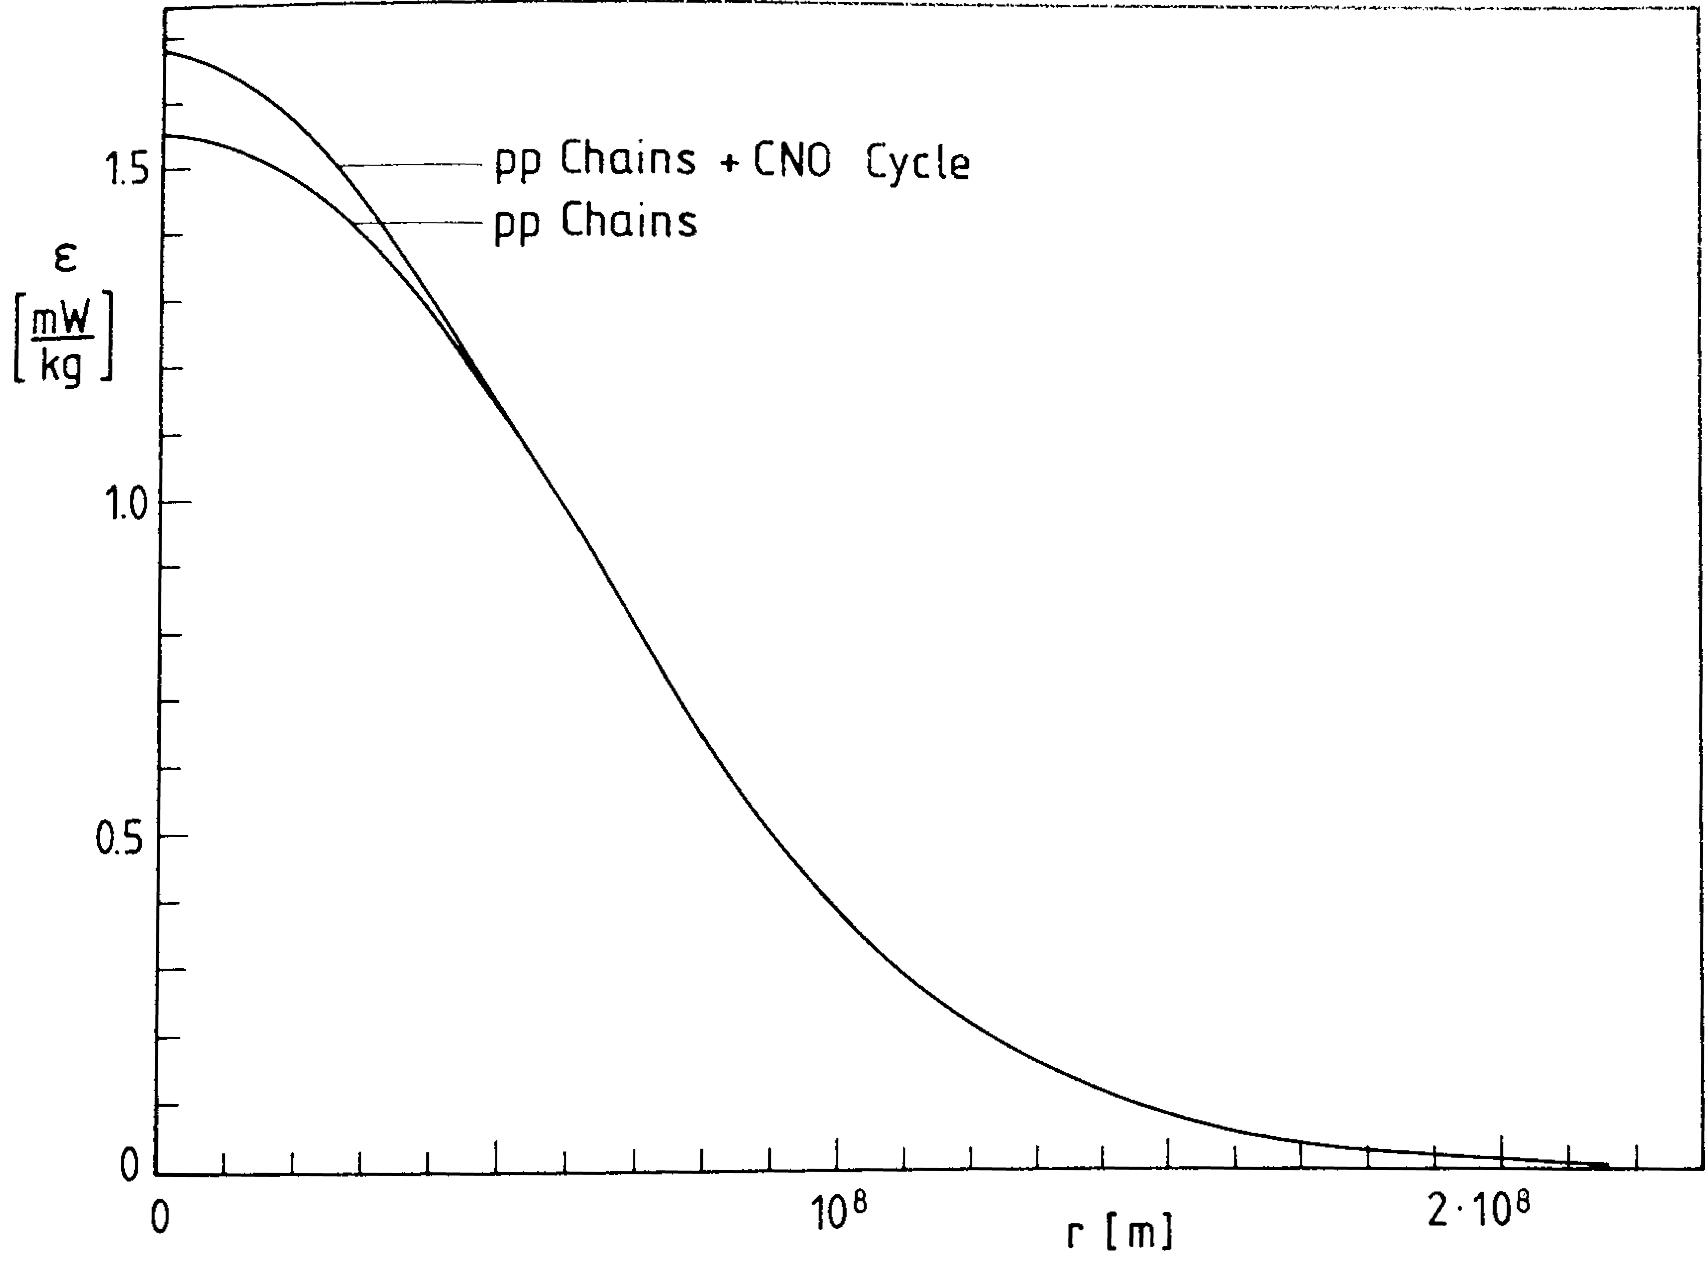
\includegraphics{watt-PPvsCNO}
    \caption{Andamento di $\epsilon$ nell'interno solare}
\end{figure}


\end{document}